\section{Parameter optimisation}
The primary goal of this experiment is to select a reasonable subset of parameters for the iris recognition experiment. Equally important, however, is the secondary goal of analysing the proposed obfuscation methods and uncertainty metrics. 

For many of the diagrams, we show only the estimated Pareto frontier derived from the sample points\todo{Define}. Note that since the points themselves are stochastic, the frontiers are likely not perfectly precise.

An overview comparing gaze estimation with mutual information (gradient based) and iris code similarity is shown in (FIGREF). The bilateral filter and non-local means exhibit large differences compared to the other methods between the two measurements, i.e. while they have lower mutual information for the same gaze error as the additive methods, they have higher iris-code similarity. This is likely caused by the fact that comparing an iris code with itself is harder when only performing some form of averaging method. The opposite is true for the mutual information measure, where the additive methods apply only high-frequency noise++. 

\begin{figure}
    \centering
    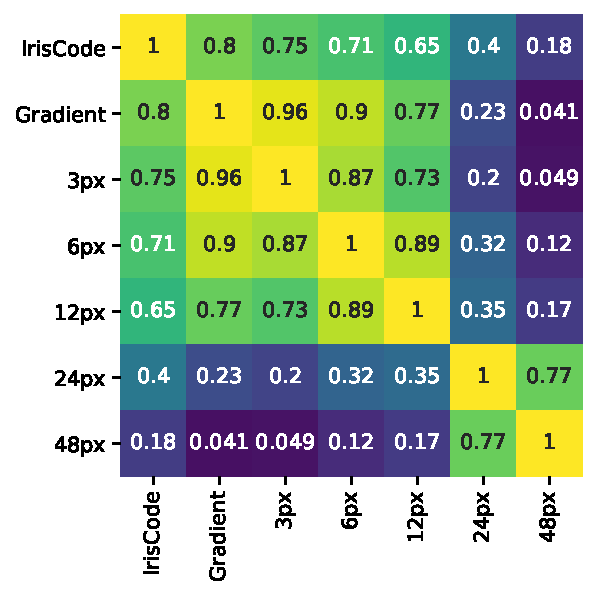
\includegraphics[width=0.8\linewidth]{figures/h1.pdf}
    \caption{Correlation matrix of the iris code and ...}
    \label{fig:h1}
\end{figure}

\begin{figure*}
    \centering
    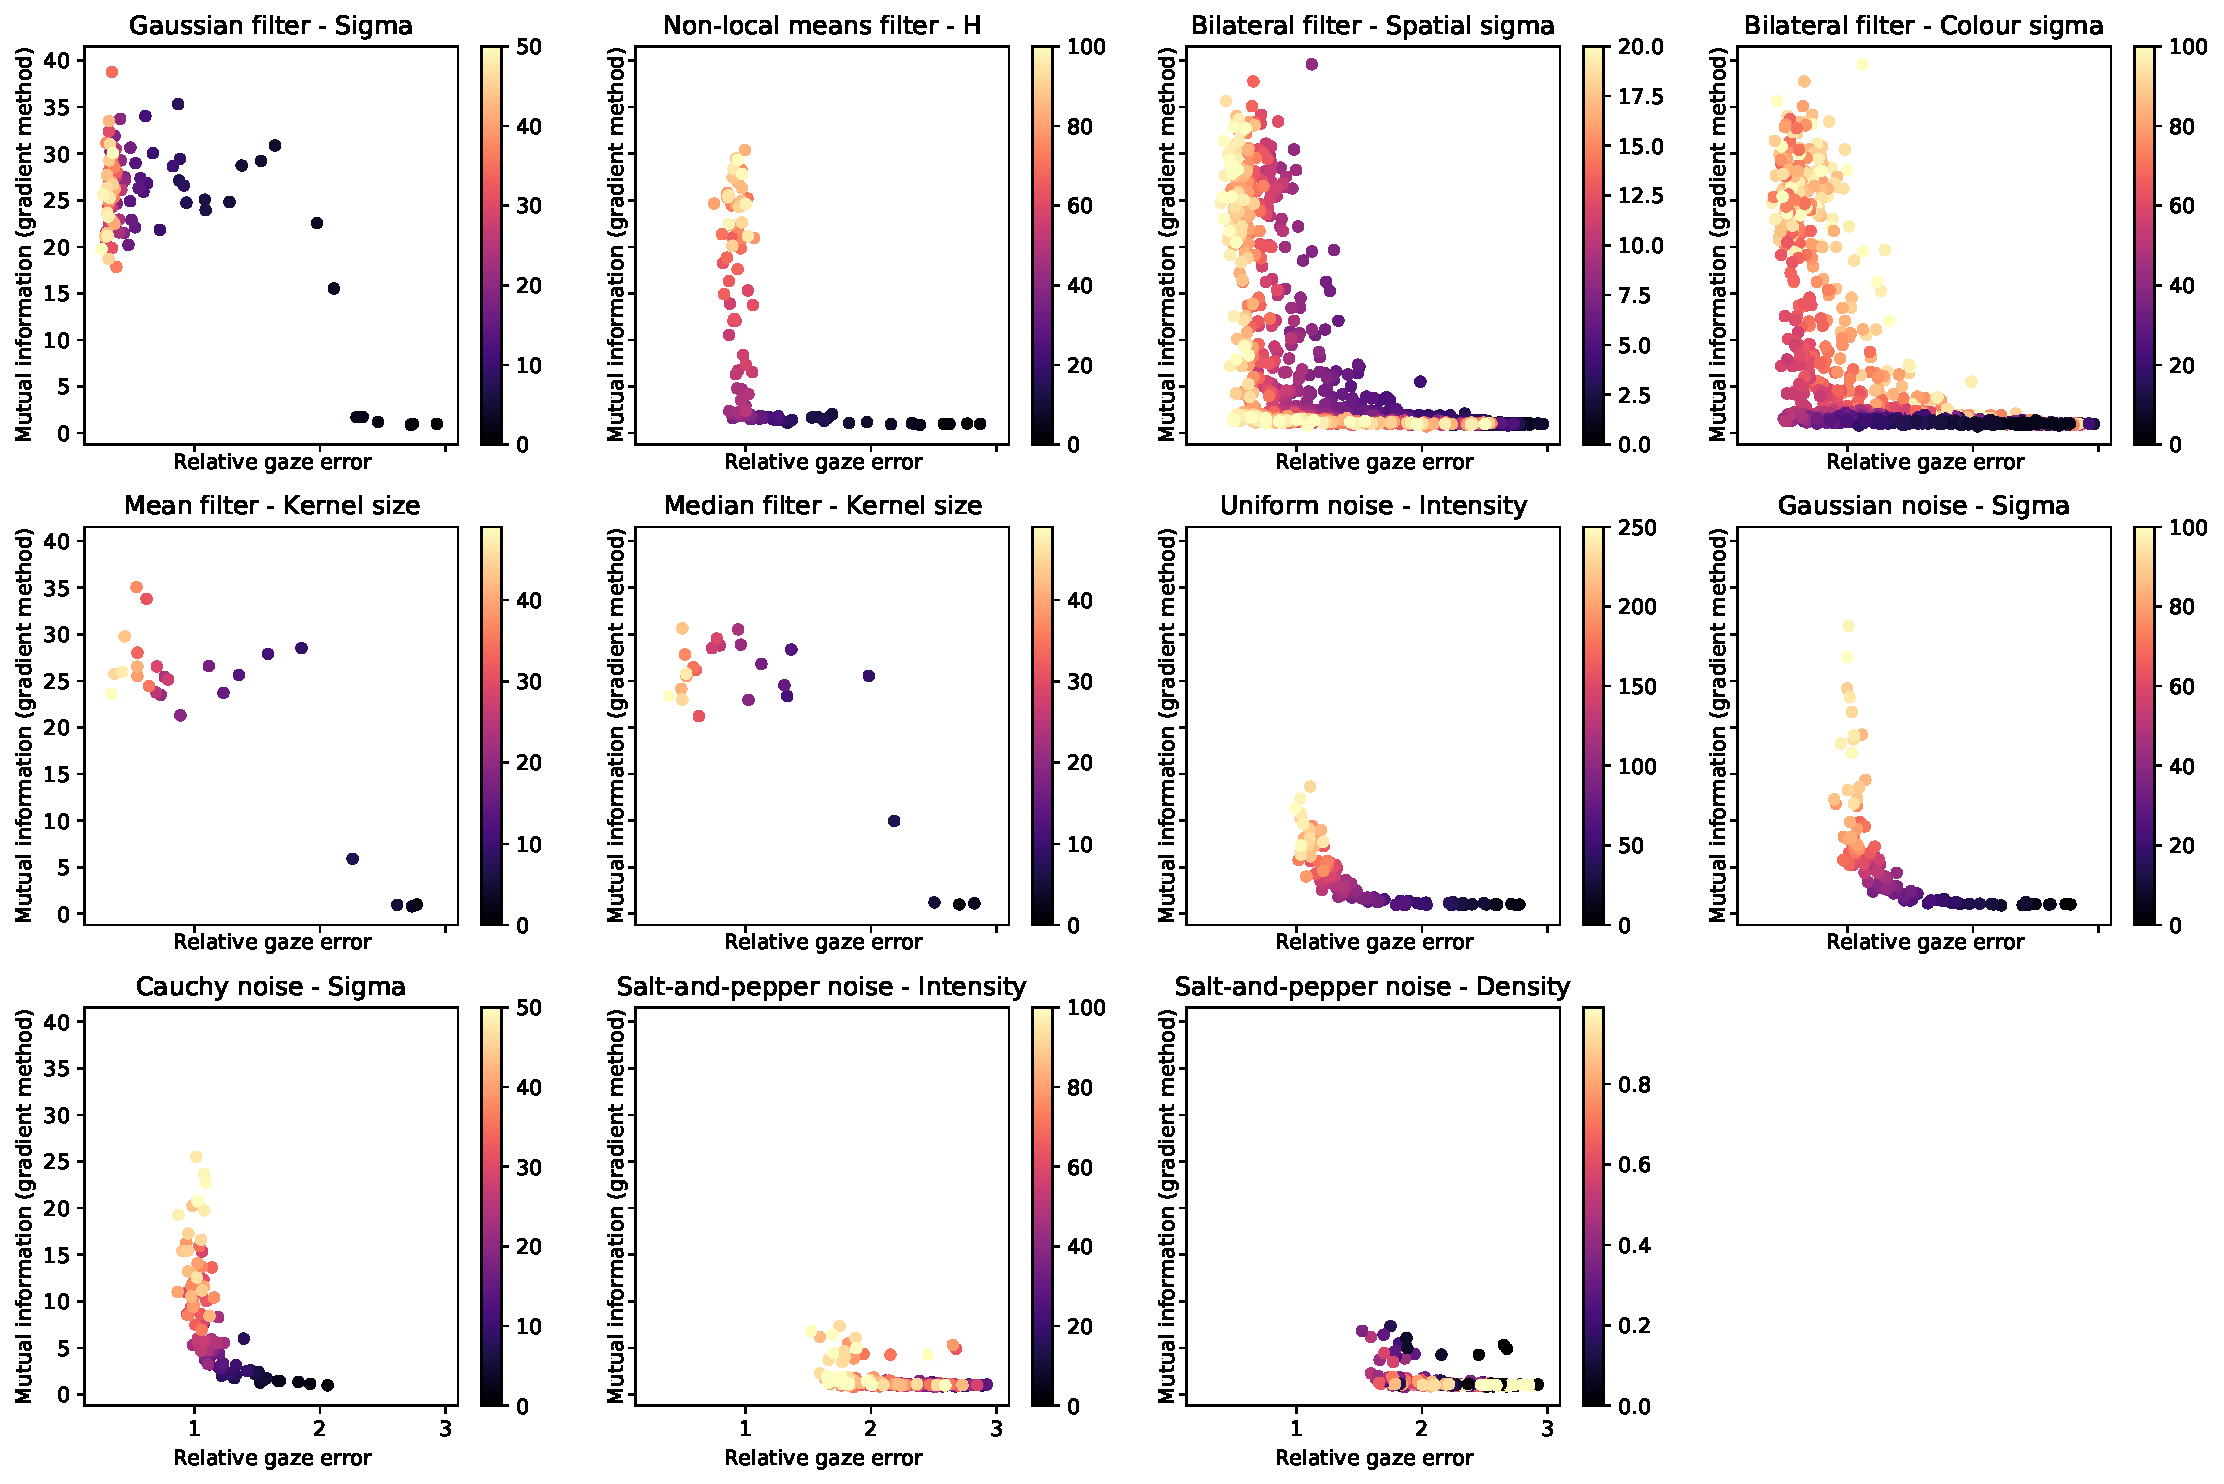
\includegraphics[width=1\textwidth]{figures/parameters.pdf}
    \caption{Correlation matrix of the iris code and ...}
    \label{fig:parameters}
\end{figure*}

\begin{figure}
    \centering
    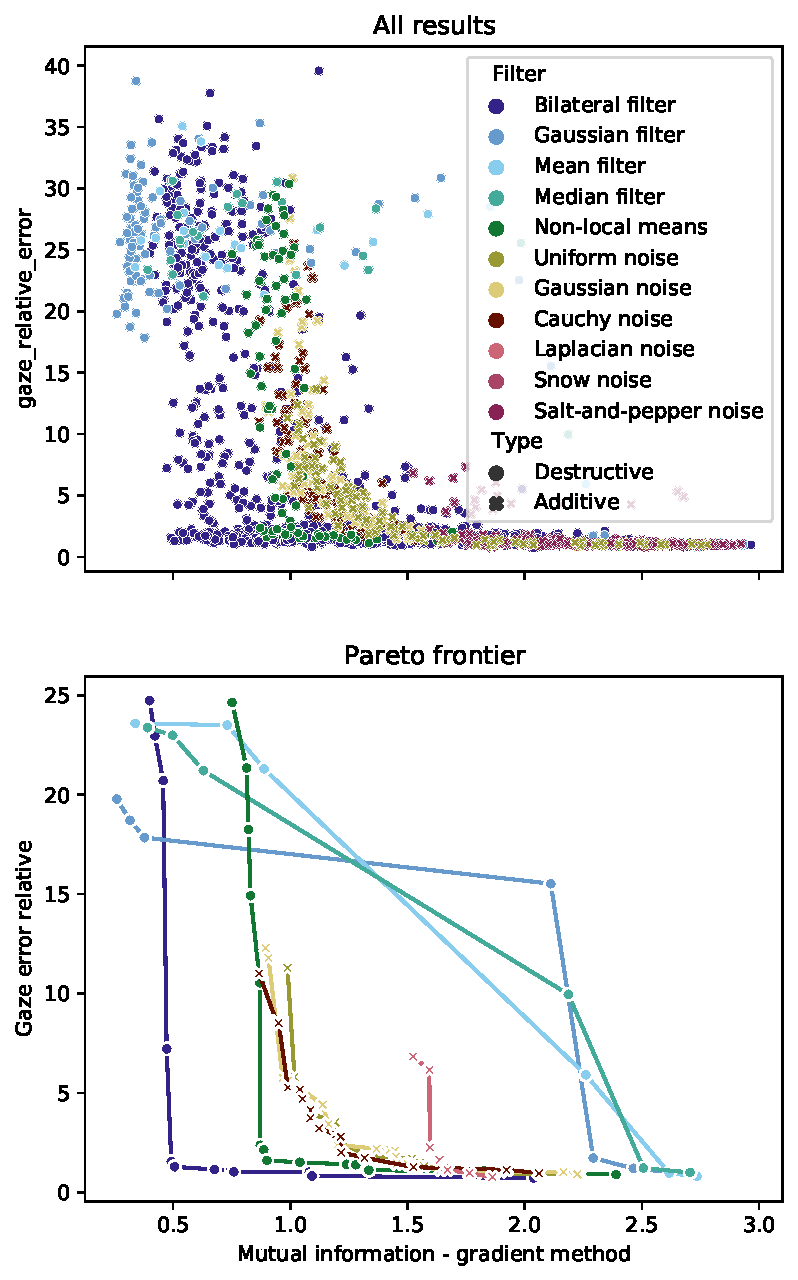
\includegraphics[width=1\linewidth]{figures/performance.pdf}
    \caption{Caption}
    \label{fig:performance}
\end{figure}

\begin{figure}
    \centering
    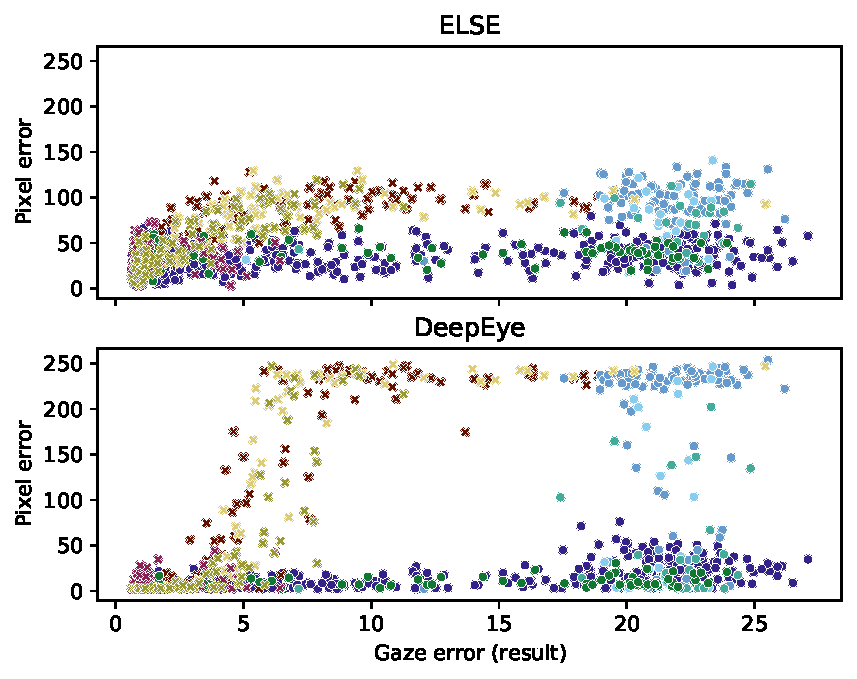
\includegraphics[width=1\linewidth]{figures/dist.pdf}
    \caption{Caption}
    \label{fig:dist}
\end{figure}

\section{Iris recognition analysis}
\begin{figure}
    \centering
    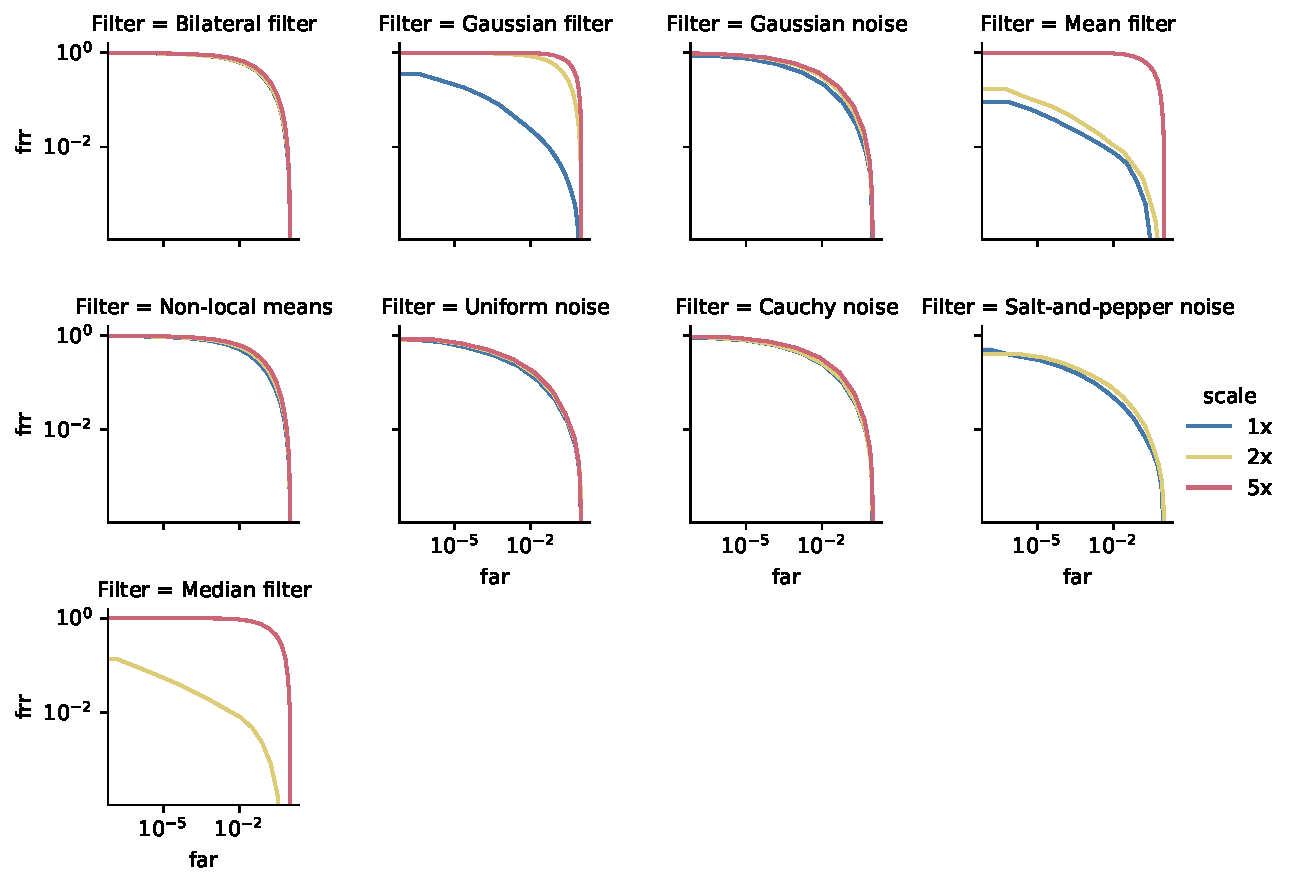
\includegraphics[width=1\linewidth]{figures/iris-comp.pdf}
    \caption{Caption}
    \label{fig:iris-comp}
\end{figure}